% Homework report template for courses lectured by Blaz Zupan.
% For more on LaTeX please consult its documentation pages, or
% read tutorials like http://tobi.oetiker.ch/lshort/lshort.pdf.
%
% Use pdflatex to produce a PDF of a report.

\documentclass[a4paper,11pt]{article}
\usepackage[slovene]{babel}
\usepackage{a4wide}
\usepackage{fullpage}
\usepackage[toc,page]{appendix}
\usepackage[pdftex]{graphicx} % for figures
\usepackage{setspace}
\usepackage{color}
\definecolor{light-gray}{gray}{0.95}
\usepackage{listings} % for inclusion of Python code
%\usepackage[colorlinks=false]{hyperref}
%\usepackage[hidelinks]{hyperref}
%\usepackage{hyperref}
\usepackage[bookmarks=true,pdfborder={0 0 0}]{hyperref}
\renewcommand{\baselinestretch}{1.2}

\setlength{\parindent}{0pt}

\setcounter{secnumdepth}{5}

\lstset{ % style for Python code, improve if needed
    language=Python,
    basicstyle=\footnotesize,
    basicstyle=\ttfamily\footnotesize\setstretch{1},
    backgroundcolor=\color{light-gray},
}

\title{Modeliranje brez\v{z}i\v{c}nih omre\v{z}ij}
\author{
    Maja Podbev"sek\\
    Peter Benko (63090004)\\
    \v{Z}iga Ham\\
    Miha Zidar (63060317)
}
\date{\today}

\begin{document}

\maketitle

\pagebreak

\tableofcontents

\pagebreak

\section{Zgledi}


%%%%%%%%%%%%%%%%%%%%%%%%%%%%%%%%%%%%%%%%%%%%%%%%%%%%%%%%%%%%%%%%%%%%%%%%%%%%

\subsection{HandOver}

V zgledu imamo naslednje module (Slika \ref{image:handover}):

\begin{itemize}
    \item dve dostopni to"cki
    \item enega odjemalca
    \item modul Configurator
\end{itemize}

Imamo le eno mo"zno konfiguracijo. Odjemalec se premika po prostoru in na dolo"ceni to"cki zamenja dostopno to"cko s katero komunicira. 

\begin{figure}[htbp]
    \begin{center}
        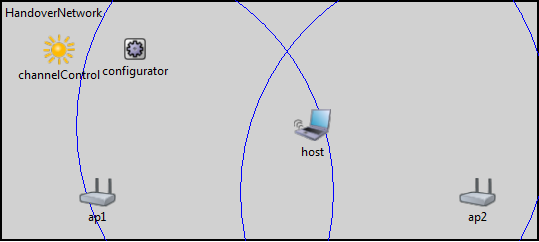
\includegraphics[scale=0.8]{img/zgledi/handover.png}
        \caption{Zgled HandOver}
        \label{image:handover}
    \end{center}
\end{figure}

%%%%%%%%%%%%%%%%%%%%%%%%%%%%%%%%%%%% HostToHost %%%%%%%%%%%%%%%%%%%%%%%%%%%%%%%%%%%%%%%%

\subsection{HostToHost}
V zgledu imamo naslednje module :

\begin{itemize}
    \item nekaj odjemalcev, od katerih en deluje kot stre"znik
    \item eno dostopno to"cko
\end{itemize}

Odjemalec in stre"znik sta povezana z brez"zi"cno povezavo.\\

Na razpolago imamo dve mo"zni konfiguraciji:

\begin{itemize}
    \item Throughput1 (Slika \ref{image:hosttohost}) – 6 odjemalcev in en stre"znik skozi dostopno to"cko
    \item General (Slika \ref{image:hosttohostgeneral}) – poljubno "stevilo odjemalcev in en stre"znik skozi dostopno to"cko
\end{itemize}

Z zgledom merimo prepustnost omre"zja pri komunikaciji odjemalca s stre"znikom. Opazujemo tudi vpliv ostalih odjemalcev na komunikacijo med zgoraj omenjenim odjemalcem in stre"znikom. Vsi akterji v omre"zju povzro"cajo "sum in s tem zmanj"sujejo prepustnost.


\begin{figure}[htbp]
    \begin{center}
        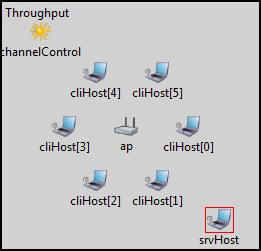
\includegraphics[scale=0.8]{img/zgledi/hosttohost.png}
        \caption{Zgled HostToHost, s konfiguracijo Throughput1}
        \label{image:hosttohost}
    \end{center}
\end{figure}

\begin{figure}[htbp]
    \begin{center}
        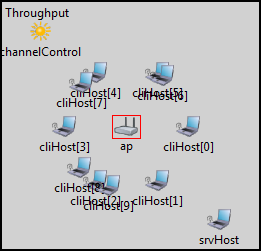
\includegraphics[scale=0.8]{img/zgledi/hostohost_general.png}
        \caption{Zgled HostToHost, s konfiguracijo General}
        \label{image:hosttohostgeneral}
    \end{center}
\end{figure}

%%%%%%%%%%%%%%%%%%%%%%%%%%%%%%%%%%%% MultiRadio %%%%%%%%%%%%%%%%%%%%%%%%%%%%%%%%%%%%%%%%

\subsection{MultiRadio}

V zgledu imamo naslednje module:

\begin{itemize}
    \item dva odjemalca
    \item dve dostopni to"cki
    \item en usmerjevalnik
    \item modul Configurator
\end{itemize}

Imamo tri konfiguracije:

\begin{itemize}
    \item Switched Wlans (Slika \ref{image:multiradioswitched}) – povezava dostopnih to"ck preko ethernet stikala
    \item Routed Wlans (Slika \ref{image:multiradiorouted}) – dva WLAN-a povezana preko usmerjevalnika z dvema brez"zi"cnima mre"znima karticama
    \item Independent Wlans (Slika \ref{image:multiradioindependent}) – dva neodvisna WLAN-a na razli"cnih radijskih kanalih
    \item General (Slika \ref{image:multiradiogeneral}) – dva neodvisna WLAN-a preko usmerjevalnika
\end{itemize}

Zgled prikazuje uporabo ve"cih brez"zi"cnih vmesnikov na enem usmerjevalniku, tako da imamo ve"c brez"zi"cnih omre"zij na razli"cnih kanalih.


\begin{figure}[htbp]
    \begin{center}
        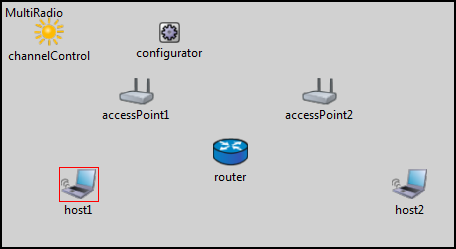
\includegraphics[scale=0.8]{img/zgledi/multiradio_general.png}
        \label{image:multiradiogeneral}
        \caption{Zgled MultiRadio, s konfiguracijo General}
    \end{center}
\end{figure}

\begin{figure}[htbp]
    \begin{center}
        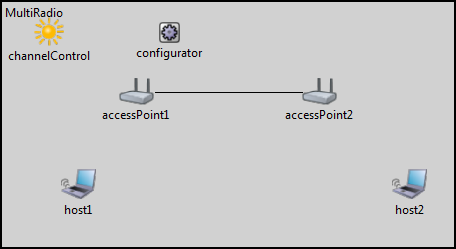
\includegraphics[scale=0.8]{img/zgledi/multiradio_switched.png}
        \caption{Zgled MultiRadio, s konfiguracijo Switched Wlans}
        \label{image:multiradioswitched}
    \end{center}
\end{figure}

\begin{figure}[htbp]
    \begin{center}
        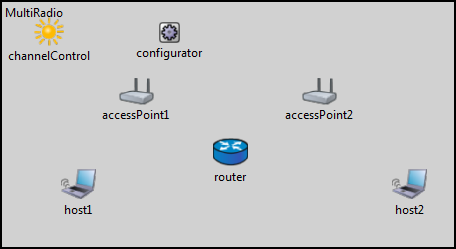
\includegraphics[scale=0.8]{img/zgledi/multiradio_routed.png}
        \caption{Zgled MultiRadio, s konfiguracijo Routed Wlans}
        \label{image:multiradiorouted}
    \end{center}
\end{figure}

\begin{figure}[htbp]
    \begin{center}
        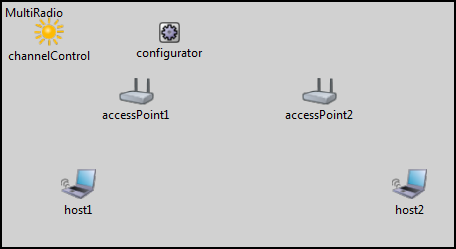
\includegraphics[scale=0.8]{img/zgledi/multiradio_independent.png}
        \caption{Zgled MultiRadio, s konfiguracijo Independent Wlans}
	\label{image:multiradioindependent}
    \end{center}
\end{figure}

%%%%%%%%%%%%%%%%%%%%%%%%%%%%%%%%%%%% Synchronized %%%%%%%%%%%%%%%%%%%%%%%%%%%%%%%%%%%%%%%%

\subsection{Synchronized}

V zgledu imamo naslednje module:
\begin{itemize}
    \item AdhocHost
    \item modul Configurator
\end{itemize}

V zgledu opazujemo anomalije pri generiranju brez"zi"cnega prometa, ki jih povzro"ca sinhrono po"siljanje paketov.

Imamo dve konfiguraciji (Slika \ref{image:synchronized}):
\begin{itemize}
    \item Synchronized – sinhrono po"siljanje paketov, pri katerem prihaja do kolizij, ki so posledica isto"casnega oddajnja paketov, zato sporo"cila niso sprejeta.
    \item NonSynchronized – nesinhrono po"siljanje paketov, kolizij je ob"cutno manj, saj vplejemo naklju"cni "casovni zamik pri po"siljanju paketov.
\end{itemize}


\begin{figure}[htbp]
    \begin{center}
        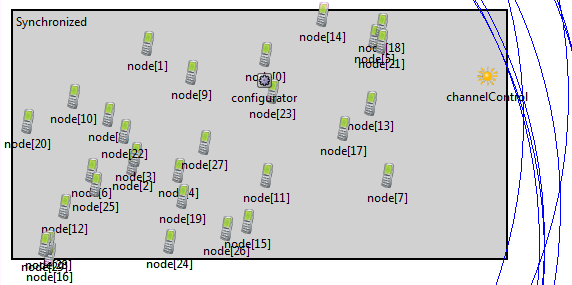
\includegraphics[scale=0.8]{img/zgledi/synchronized_sync.png}
        \caption{Zgled Synchronized, s sinhrono in asinhrono konfiguracijo}
	\label{image:synchronized}
    \end{center}
\end{figure}



%%%%%%%%%%%%%%%%%%%%%%%%%%%%%%%%%%%% Throughput %%%%%%%%%%%%%%%%%%%%%%%%%%%%%%%%%%%%%%%%

\subsection{Throughput}

V zgledu imamo naslednje module:
\begin{itemize}
    \item nekaj mobilnih odjemalcev
    \item eno dostopno to"cko
\end{itemize}

Z zgeldom merimo prepustnost omre"zja med ve"cinimi odjemalci in dostopno to"cko. Prepustnost je vedno manj"sa od teoreti"cne maksimalne, saj si odjemalci delijo medij in prihaja do kolizij. Odjemalci in dostopna to"cka so konfigurirani tako, da vsak odjemalec sli"si vse ostale odjemalce.\\

Imamo dva ni"cina konfiguracije:

\begin{itemize}
    \item Throughput1 (Slika \ref{image:throughputthr1}) – en odjemalec do dostopne to"cke
    \item Throughput2 (Slika \ref{image:throughputthr2}) – trije odjemalci do dostopne to"cke
    \item General (Slika \ref{image:throughputgeneral}) – poljubno "stevilo odjemalcev do dostopne to"cke
\end{itemize}

Prepustnost merimo s ``Sink'' podmodulom dostopne to"cke.

Vsi zgledi vsebujejo tudi modul ChannelControl. Moduli so podrobno opisani v analizi zgleda Lan80211.


\begin{figure}[htbp]
    \begin{center}
        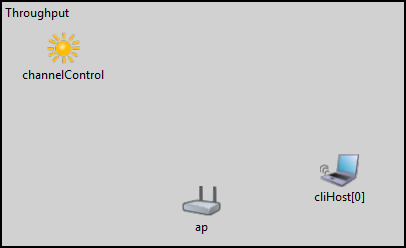
\includegraphics[scale=0.8]{img/zgledi/throughput_thr1.png}
        \caption{Zgled Throughput, s konfiguracijo Throughput1}
	\label{image:throughputthr1}
    \end{center}
\end{figure}


\begin{figure}[htbp]
    \begin{center}
        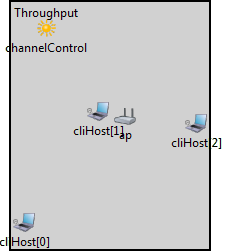
\includegraphics[scale=0.8]{img/zgledi/throughput_thr2.png}
        \caption{Zgled Throughput, s konfiguracijo Throughput2}
	\label{image:throughputthr2}
    \end{center}
\end{figure}

\begin{figure}[htbp]
    \begin{center}
        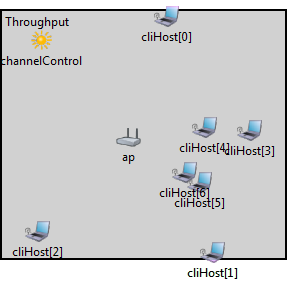
\includegraphics[scale=0.8]{img/zgledi/throughput_general.png}
        \caption{Zgled Throughput, s konfiguracijo General}
	\label{image:throughputgeneral}
    \end{center}
\end{figure}



%%%%%%%%%%%%%%%%%%%%%%%%%%%%%%%%%%%% 80211 %%%%%%%%%%%%%%%%%%%%%%%%%%%%%%%%%%%%%%%%


\section{Lan80211}


\begin{figure}[htbp]
    \begin{center}
        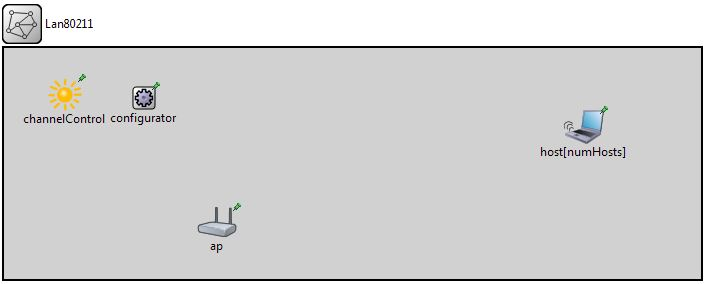
\includegraphics[scale=0.8]{img/lan80211.jpg}
        \caption{Shema modela 802.11}
	\label{image:lan80211}
    \end{center}
\end{figure}


\subsection{Gradniki}

\subsubsection{Access Point}
\label{description:acceesspoint}

oziroma dostopna to"cka je enota, ki lahko sprejema in oddaja brez"zi"cne signale. Hrani tudi tabelo vseh enot, ki so trenutno povezana na njo. Ima ena "zi"cna vrata v svetovni splet, ter na drugi strani anteno za brez"zi"cno komunikacijo. Vmes podatke posreduje relacijska enota. 

\begin{figure}[htbp]
    \begin{center}
        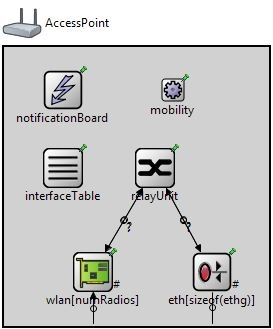
\includegraphics[scale=0.8]{img/ap.jpg}
        \caption{Shema dostopne to"cke}
	\label{image:ap}
    \end{center}
\end{figure}


\paragraph{interfaceTable}
\label{description:interfacetable}

je objekt preprostega modula InterfaceTable. Nima nikaker"snih vrat in posledi"cno tudi ne obdelave sporo"cil. Uporablja se zgolj z uporabo funkcij. Deluje kot slovar za prevajanje, ali "se bole, kot tabela za prevajanje vseh priklju"cenih naprav. Obdeluje se dinami"cno, ob priklopu se nova naprava registrira v tabelo in poskrbi za vnose v routing tabele (IRoutingTable in IRoutingTable6). V interfaceTable se vna"sajo InterfaceEntry-ji, ki vsebujejo podatke, kot so: interfaceId(unikadtna identifikacijska "stevilka, ki zaznamuje vnos), id vhodnih in izhodnih vrat naslovnika, MTU, pasovno "sirino, MAC naslov, trenutno stanje (up/down) ter podatke kaj podpira (broadcast, multicast, point to point, loopback).



\paragraph{notificationBoard}
\label{description:notificationboard}

je objekt preprostega mudula ``notificationBoard'', s katerim realiziramo vmesnik za sprejemanje in zazpe"cevanje obvestil. ob prijavise v tem modulu vsak odjemalec ``prijavi'' na kategorije, ki se jih ti"cejo. "ce "zeli katerikoli od odjemalcev poslati sporo"cilo mora zahtevo najprej predati notificationBoard-u, ki potem razpo"slje tosporo"cilo vsem primernim odjemalcem, torej takim, ki so naro"ceni na specifi"cno ``kategorijo''.

\paragraph{wlan[]}
\label{description:wlan}

predstavlja brez"zi"cno mre"zno kartico (IWirelessNic - Wireless Network Interface Controller, po protokolu implementiranem v Ieee80211Nic), ki je raz"siritev modula mre"znih kartic ('INic'). Gre za eno kartico, na kateri vsak vnos v tabelo wlan[] predstavlja eno anteno oz. oddajnik. Vsebovani moduli wlan[] enote so prikazani na Sliki \ref{image:shema80211nic}. Modul Ieee80211Radio je fizi"cni nivo wlan-a. Oddaja in sprejema brez"zi"cne signale ter jih posreduje enoti 'mac' (modul Ieee80211Mac). Mac za sprejeti paket skrbi, da se je pravilno sprejel, oz. da se bo pravilno poslal. Pri po"siljanju potrebuje vsa polja paketa izpolnjena. Sam zna zapolniti le izvorni MAC naslov paketka. Enota mgmt (modul IIeee80211Mgmt) posreduje pakete med nivoji ter dodaja funkcionalnost agenta. Agent (preprost modul Ieee80211AgentSTA) skrbi za skeniranje kanalov, antentikacijo ter povezovanje. Deluje v dveh na"cinih skeniranja: aktivno ter pasivno. Agentu (modul Ieee80211AgentSTA) lahko podamo spisek kanalov, ki naj jih preveri, zamik med skeniranji, minimalni "cakalni "cas, ki ga mora porabiti na dolo"cenem kanalu med aktivnim skeniranjem, "cas ki ga porabi na vsakemkanalu ob pasivnem skeniranju, avtentikacijski timeout ter timeout za povezovanje. Agentu dolo"ca tudi SSID, ki ga bo wlan[] ogla"seval. Input in output zanki sta realizirani zgolj za simulacijo, saj sta zelo primerni za umetno ustvarjanje dolo"cenih napak na omre"zju.

\begin{figure}[htbp]
    \begin{center}
        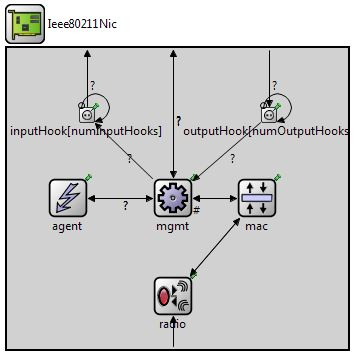
\includegraphics[scale=0.8]{img/radio.jpg}
        \caption{Shema dostopne to"cke}
	\label{image:shema80211nic}
    \end{center}
\end{figure}


\paragraph{relayUnit}
\label{description:relayunit}

je objekt modula IMACRelayUnit, ki skrbi za posredovanje in obdelavo prejetih okvirjev. Ima vhodna in izhodna vrata od/k ni"zjim plastem, skozi katera na eni strani komunicira z o"zi"cenim omre"zjem in na drugi strani z brez"zi"cnim omre"zjem. S pomo"cjo tabele naslovov usmerja pakete na pravilna vrata in oz. pravilne MAC naslove. Skrbi tudi za sve"zino tabele naslovov, saj ima omejeno velikost. Ko se le-ta zapolni, bo iz nje izbrisan najstarej"si vnos.

\paragraph{eth[]}
\label{description:eth}

sloni na preprostem modulu EtherMACFullDuplex, ki je preprostej"sa oblika IEtherMAC. Skrbi za o"zi"ceno komunikacijo. Prav tako kot wlan[] ne izvaja nikakr"sne enkapsulacije/dekapsulacije, za to posreduje okvirje vi"sjim plastem. Pri po"siljanju se vsi prejeti paketi (od vi"sjih plasti) postavijo v vrsto, kjer po"cakajo, da je oddajnik prost. Ko je mo"zno jih takoj po"slje. V paketu morajo biti vsa polja "ze izpolnjena, le izvorni MAC se bo tu naknadko dodal, "ce je polje prazno. Pri sprejemanju paketov (iz omre"zja) opravi najprej CRC check, pri "cimer so paketi z napako zavr"zeni, in nato posreduje pakete naprej vi"sji plasti.


\paragraph{mobility}
\label{description:mobility}

zagotavlja zgolj vizualno realizacijo gibljivih modelov na shemi omre"zja - v tem primeru dostopne to"cke, gi pa je stacionarna, zato vra"ca lastnosti getCurrentPosition in getCurrentSpeed enaki 0.


\subsubsection{WirelessHost}
\label{description:wirelesshost}



\begin{figure}[htbp]
    \begin{center}
        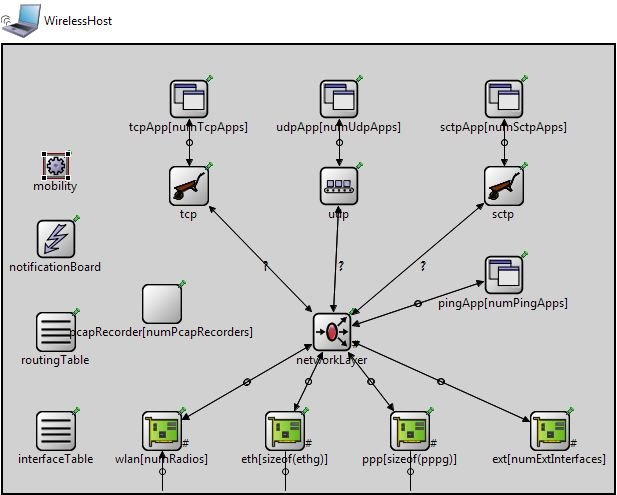
\includegraphics[scale=0.8]{img/host.jpg}
        \caption{Shema modula WirelessHost}
	\label{image:wirelesshost}
    \end{center}
\end{figure}


\paragraph{Mre"zne kartice}
\label{description:mreznekartice}

\begin{enumerate}
    \item \textbf{wlan[]} zagotavlja brez"zi"cno povezljivost naprave, s pomo"cjo modula Ieee80211Nic, enako kot je opisano pod to"cko \ref{description:wlan} - wlan[] dostopne to"cke.


    \item \textbf{eth[]} zagotavlja o"zi"ceno povezljivost s pomo"cjo modula EthernetInterface. Pri lan80211 se ne uporablja, saj vsa komunikacija poteka preko wlan[] povezave.

    \item \textbf{ppp} zagotavlja point-to-point povezljivost, prav tako kot eth[] se pri lan80211 ne uporablja.

    \item \textbf{ext} omogo"ca realizacijo zunanjih mre"znih kartic.

\end{enumerate}


\paragraph{NetworkLayer}
\label{description:networklayer}


\begin{figure}[htbp]
    \begin{center}
        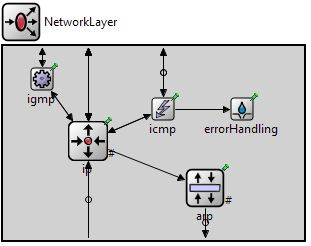
\includegraphics[scale=0.8]{img/network.jpg}
        \caption{Shema modula NetworkLayer}
	\label{image:wirelesshost}
    \end{center}
\end{figure}

\begin{enumerate}
    \item \textbf{ip} je implementiran s preprostim modulom IPv4. Izpolnjuje IPv4 en-/de-kapsulacijo paketa. Ko je sprejet paket sprejet, ga odpre in odstranjene podatke predavi"sji plasti v obliki IPv4ControlInfo, izlu"s"cene podatke pa preda kot cMessage. V obratni smeri je pri"cakovano, da vi"sja plast poleg sporo"cila poda tudi izpolnjen IPv4ControlInfo. Ob po"siljanji se preveri izhodni port v RoutingTable ter naslov naslednjega skoka paketka.

    \item \textbf{icmp} skrbi za implementacijo ICMP-ja. Sprejema ICMP sporo"cila in jih procesira. Za prejete zahtevke ustvari odgovore ter jih predatakoj nazaj v IPv4 enkapsulacijo. Opazimo da se zunanji 'ping' zahtevki obdelajo na mre"zni plasti. "ce sprejme ICMP odgovor, ga izlu"s"ci is ICMP okvirja, ter preda vi"sji plasti. "ce sprejme ping zahtevek z vi"sje plasti, ga enkapsulira v ISMP okvir ter preda IPv4 enoti.

    \item \textbf{igmp} po"silja obvestila o pripadnosti multicast skupinam odjemalca, na strani routerja pa ta obvestila procesira.

    \item \textbf{arp} implementira protokol ARP za IPv4 in 6-bajtni MAC.

    \item \textbf{errorHandling} procesira sporo"cila o napakah od ostalih modulov.

\end{enumerate}



\paragraph{Protokoli}
\label{description:Protokoli}


\begin{enumerate}

    \item \textbf{tcp} realizira TCP protokol (preko ITCP modula), preko katerega lahko aplikacije vzpostavljajo TCP povezave. Za vzpostavitev povezave mora aplikacija protokolni enoti najprej poslati zahtevek za vzpostavitev aktivne oz. pasivne povezave preko controlInfo lastnosti cMessage-a. Za po"siljanjepaketov mora aplikacija paketku nastaviti TCP\_C\_SEND kot vrsto sporo"cila ter prilo"ziti TCPSendCommand kontrolne informacije. Za zaprtje povezave aplikacija po"slje TCP\_C\_CLOSE vrsto sporo"cila z TCPSend kontrolnimi informacijami, da se ve katero povezavo se zapira. Modula tudi obve"s"ca aplikacijo o vseh velikih spremembah v povezavi (povezava vzpostavljena, prekinjena, zavrnjena, izgubljena...).

    \item \textbf{udp} implementira UDP protokol (preko IUDP modula). Za po"siljanje aplikacija zkolj preda paket udp enoti s prilo"zenim UDPControlInfo objektom. Za prejemanje mora aplikacija najprej 'rezervirati' dolo"cen port. To stori z sporo"cilom vrste UDP\_C\_BIND s prilo"zenim UDPControlInfo, ki ima izpolnjeno srcPort polje. 

    \item \textbf{sctp} vmesnik za realizacijo SCTP protokola.

\end{enumerate}






\paragraph{Aplikacije}
\label{description:aplikacije}

So okvirni primeri aplikacij, ki imajo realizirana zgolj vrata, klju"cna za delovanje aplikacije s primernim protokolom. 



\paragraph{Ostalo}
\label{description:ostalo}


\begin{enumerate}
    \item \textbf{routingTable} hrani routingTable. V njej se hranijo podatki za usmerjanje paketkov. V programu se navezujena dokument 'routingFile'.

    \item \textbf{pcapRecorder} je implementiran za bele"zenje, katere okvirje po"siljajo ostali moduli znotraj iste enote. Izbiramo lahko katere module se bele"zi ter katerim signalom se sledi ter dodajamo.

    \item \textbf{interfaceTable} opis v \ref{description:interfacetable}

    \item \textbf{notificationBoard} opis v \ref{description:notificationboard} 

    \item \textbf{mobility} opis v \ref{description:mobility}
\end{enumerate}




\subsubsection{ChannelControl}

Vsako omre"zje z mobilnimi napravami ali brez"zi"cnimi omre"zji. Glede na lokacijo elementov dolo"ca kateri so v dosegu, da lahko komunicirajo med sabo oz. povzro"cajo inteferenco. Te podatke potem uporabijo brez"zi"cne enote, da lahko dolo"cajo s katerimi enotami lahko komunicirajo.

\subsubsection{IPv4NetworkConfigurator}

Ta modula dodeli IP naslove (lahko ro"cno ali avtomati"cno) in vzpostavi stati"cno usmerjanjepo IPv4 omre"zju. Module, ki predstavljajo omre"zne enote prepoznava po @node lastnosti, zato jo morajo vse enote vsebovati. Prav tako jeod njih pri"cakovano, da imajo vsaka svon InterfaceTable, za routerje pa "se RoutingTable. 

\section{Na\v{s} model}


\subsection{Opis}

\subsection{Meritve}




\end{document}

